\documentclass[twoside]{book}

% Packages required by doxygen
\usepackage{fixltx2e}
\usepackage{calc}
\usepackage{doxygen}
\usepackage[export]{adjustbox} % also loads graphicx
\usepackage{graphicx}
\usepackage[utf8]{inputenc}
\usepackage{makeidx}
\usepackage{multicol}
\usepackage{multirow}
\PassOptionsToPackage{warn}{textcomp}
\usepackage{textcomp}
\usepackage[nointegrals]{wasysym}
\usepackage[table]{xcolor}

% Font selection
\usepackage[T1]{fontenc}
\usepackage[scaled=.90]{helvet}
\usepackage{courier}
\usepackage{amssymb}
\usepackage{sectsty}
\renewcommand{\familydefault}{\sfdefault}
\allsectionsfont{%
  \fontseries{bc}\selectfont%
  \color{darkgray}%
}
\renewcommand{\DoxyLabelFont}{%
  \fontseries{bc}\selectfont%
  \color{darkgray}%
}
\newcommand{\+}{\discretionary{\mbox{\scriptsize$\hookleftarrow$}}{}{}}

% Page & text layout
\usepackage{geometry}
\geometry{%
  a4paper,%
  top=2.5cm,%
  bottom=2.5cm,%
  left=2.5cm,%
  right=2.5cm%
}
\tolerance=750
\hfuzz=15pt
\hbadness=750
\setlength{\emergencystretch}{15pt}
\setlength{\parindent}{0cm}
\setlength{\parskip}{3ex plus 2ex minus 2ex}
\makeatletter
\renewcommand{\paragraph}{%
  \@startsection{paragraph}{4}{0ex}{-1.0ex}{1.0ex}{%
    \normalfont\normalsize\bfseries\SS@parafont%
  }%
}
\renewcommand{\subparagraph}{%
  \@startsection{subparagraph}{5}{0ex}{-1.0ex}{1.0ex}{%
    \normalfont\normalsize\bfseries\SS@subparafont%
  }%
}
\makeatother

% Headers & footers
\usepackage{fancyhdr}
\pagestyle{fancyplain}
\fancyhead[LE]{\fancyplain{}{\bfseries\thepage}}
\fancyhead[CE]{\fancyplain{}{}}
\fancyhead[RE]{\fancyplain{}{\bfseries\leftmark}}
\fancyhead[LO]{\fancyplain{}{\bfseries\rightmark}}
\fancyhead[CO]{\fancyplain{}{}}
\fancyhead[RO]{\fancyplain{}{\bfseries\thepage}}
\fancyfoot[LE]{\fancyplain{}{}}
\fancyfoot[CE]{\fancyplain{}{}}
\fancyfoot[RE]{\fancyplain{}{\bfseries\scriptsize Generated by Doxygen }}
\fancyfoot[LO]{\fancyplain{}{\bfseries\scriptsize Generated by Doxygen }}
\fancyfoot[CO]{\fancyplain{}{}}
\fancyfoot[RO]{\fancyplain{}{}}
\renewcommand{\footrulewidth}{0.4pt}
\renewcommand{\chaptermark}[1]{%
  \markboth{#1}{}%
}
\renewcommand{\sectionmark}[1]{%
  \markright{\thesection\ #1}%
}

% Indices & bibliography
\usepackage{natbib}
\usepackage[titles]{tocloft}
\setcounter{tocdepth}{3}
\setcounter{secnumdepth}{5}
\makeindex

% Hyperlinks (required, but should be loaded last)
\usepackage{ifpdf}
\ifpdf
  \usepackage[pdftex,pagebackref=true]{hyperref}
\else
  \usepackage[ps2pdf,pagebackref=true]{hyperref}
\fi
\hypersetup{%
  colorlinks=true,%
  linkcolor=blue,%
  citecolor=blue,%
  unicode%
}

% Custom commands
\newcommand{\clearemptydoublepage}{%
  \newpage{\pagestyle{empty}\cleardoublepage}%
}

\usepackage{caption}
\captionsetup{labelsep=space,justification=centering,font={bf},singlelinecheck=off,skip=4pt,position=top}

%===== C O N T E N T S =====

\begin{document}

% Titlepage & ToC
\hypersetup{pageanchor=false,
             bookmarksnumbered=true,
             pdfencoding=unicode
            }
\pagenumbering{alph}
\begin{titlepage}
\vspace*{7cm}
\begin{center}%
{\Large Laboratorio No.2 }\\
\vspace*{1cm}
{\large Generated by Doxygen 1.8.14}\\
\end{center}
\end{titlepage}
\clearemptydoublepage
\pagenumbering{roman}
\tableofcontents
\clearemptydoublepage
\pagenumbering{arabic}
\hypersetup{pageanchor=true}

%--- Begin generated contents ---
\chapter{Hierarchical Index}
\section{Class Hierarchy}
This inheritance list is sorted roughly, but not completely, alphabetically\+:\begin{DoxyCompactList}
\item \contentsline{section}{figura}{\pageref{classfigura}}{}
\begin{DoxyCompactList}
\item \contentsline{section}{circulo}{\pageref{classcirculo}}{}
\item \contentsline{section}{rectangulo}{\pageref{classrectangulo}}{}
\item \contentsline{section}{triangulo}{\pageref{classtriangulo}}{}
\end{DoxyCompactList}
\end{DoxyCompactList}

\chapter{Class Index}
\section{Class List}
Here are the classes, structs, unions and interfaces with brief descriptions\+:\begin{DoxyCompactList}
\item\contentsline{section}{\hyperlink{classcirculo}{circulo} }{\pageref{classcirculo}}{}
\item\contentsline{section}{\hyperlink{classfigura}{figura} }{\pageref{classfigura}}{}
\item\contentsline{section}{\hyperlink{classrectangulo}{rectangulo} }{\pageref{classrectangulo}}{}
\item\contentsline{section}{\hyperlink{classtriangulo}{triangulo} }{\pageref{classtriangulo}}{}
\end{DoxyCompactList}

\chapter{Class Documentation}
\hypertarget{classcirculo}{}\section{circulo Class Reference}
\label{classcirculo}\index{circulo@{circulo}}


Inheritance diagram for circulo\+:\nopagebreak
\begin{figure}[H]
\begin{center}
\leavevmode
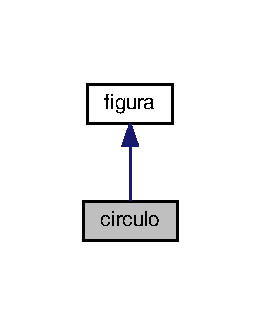
\includegraphics[width=125pt]{classcirculo__inherit__graph}
\end{center}
\end{figure}


Collaboration diagram for circulo\+:\nopagebreak
\begin{figure}[H]
\begin{center}
\leavevmode
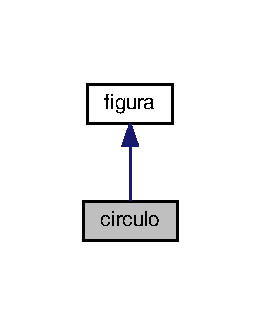
\includegraphics[width=125pt]{classcirculo__coll__graph}
\end{center}
\end{figure}
\subsection*{Public Member Functions}
\begin{DoxyCompactItemize}
\item 
\hyperlink{classcirculo_a5a035141e32d31d290d9a707894ec418}{circulo} (double radio, int id, std\+::string nombre, std\+::string color)
\begin{DoxyCompactList}\small\item\em Función utilizada, para llamar al constructor de la clase circulo. \end{DoxyCompactList}\item 
\mbox{\Hypertarget{classcirculo_a4b175bd2b25be1def566c1f84e13932c}\label{classcirculo_a4b175bd2b25be1def566c1f84e13932c}} 
\hyperlink{classcirculo_a4b175bd2b25be1def566c1f84e13932c}{$\sim$circulo} ()
\begin{DoxyCompactList}\small\item\em Función utilizada, para llamar al destructor de circulo. \end{DoxyCompactList}\item 
sf\+::\+Circle\+Shape \hyperlink{classcirculo_ab67562f2a62b5de13b4208b8aa83a0fb}{dibujar} (sf\+::\+Render\+Window $\ast$rW)
\begin{DoxyCompactList}\small\item\em Función utilizada, para llamar al metodo que dibuja circulo. \end{DoxyCompactList}\item 
\mbox{\Hypertarget{classcirculo_ae229e0665a893888c4c35f53ba407dda}\label{classcirculo_ae229e0665a893888c4c35f53ba407dda}} 
void \hyperlink{classcirculo_ae229e0665a893888c4c35f53ba407dda}{c\+\_\+area} ()
\begin{DoxyCompactList}\small\item\em Función heredada, para llamar al método que calcula el área del circulo, multiplicando el radio por si mismo y por PI, definido en la clase. \end{DoxyCompactList}\item 
\mbox{\Hypertarget{classcirculo_a1e6b523f98f276c780a36cd29f25a15e}\label{classcirculo_a1e6b523f98f276c780a36cd29f25a15e}} 
void \hyperlink{classcirculo_a1e6b523f98f276c780a36cd29f25a15e}{perimetro} ()
\begin{DoxyCompactList}\small\item\em Función heredada, para calcular el perímetro del circulo. \end{DoxyCompactList}\item 
\mbox{\Hypertarget{classcirculo_a855a548d7426a8272171889d661032ab}\label{classcirculo_a855a548d7426a8272171889d661032ab}} 
void \hyperlink{classcirculo_a855a548d7426a8272171889d661032ab}{info} ()
\begin{DoxyCompactList}\small\item\em Función heredada, para imprimir la info del circulo a través de los parámetros miembros de la clase. \end{DoxyCompactList}\item 
\mbox{\Hypertarget{classcirculo_a2a70c0e9468e8450871b9704aeb516cf}\label{classcirculo_a2a70c0e9468e8450871b9704aeb516cf}} 
void \hyperlink{classcirculo_a2a70c0e9468e8450871b9704aeb516cf}{operator$\sim$} ()
\begin{DoxyCompactList}\small\item\em Función operador, para sobreescribir el simbolo $\sim$. \end{DoxyCompactList}\item 
\mbox{\Hypertarget{classcirculo_a46e8b7ec1f88b0f9392382b9b99428fb}\label{classcirculo_a46e8b7ec1f88b0f9392382b9b99428fb}} 
void \hyperlink{classcirculo_a46e8b7ec1f88b0f9392382b9b99428fb}{operator!} ()
\begin{DoxyCompactList}\small\item\em Función operador, para sobreescribir el simbolo !. \end{DoxyCompactList}\item 
\hyperlink{classcirculo}{circulo} $\ast$ \hyperlink{classcirculo_a4dc6891872873a86791f3777c74d8aad}{operator=} (const \hyperlink{classcirculo}{circulo} $\ast$t)
\begin{DoxyCompactList}\small\item\em metodo operador para un pointer de tipo circulo, para sobreescribir el simbolo =. \end{DoxyCompactList}\item 
\mbox{\Hypertarget{classcirculo_a4a943b20d7e86555fb5da55b5177f87e}\label{classcirculo_a4a943b20d7e86555fb5da55b5177f87e}} 
int \hyperlink{classcirculo_a4a943b20d7e86555fb5da55b5177f87e}{get\+\_\+num\+\_\+circulos} ()
\begin{DoxyCompactList}\small\item\em metodo get\+\_\+num\+\_\+circulos para obtener el numero de instancias de la clase circulo. \end{DoxyCompactList}\end{DoxyCompactItemize}
\subsection*{Public Attributes}
\begin{DoxyCompactItemize}
\item 
\mbox{\Hypertarget{classcirculo_a892b0a66e25aa6686fbfd4e1c2a5d43a}\label{classcirculo_a892b0a66e25aa6686fbfd4e1c2a5d43a}} 
sf\+::\+Circle\+Shape {\bfseries circle}
\end{DoxyCompactItemize}
\subsection*{Static Public Attributes}
\begin{DoxyCompactItemize}
\item 
\mbox{\Hypertarget{classcirculo_a2b1fcb1385194d5d1b11ad3328727ec8}\label{classcirculo_a2b1fcb1385194d5d1b11ad3328727ec8}} 
static int {\bfseries num\+\_\+circulos}
\end{DoxyCompactItemize}


\subsection{Constructor \& Destructor Documentation}
\mbox{\Hypertarget{classcirculo_a5a035141e32d31d290d9a707894ec418}\label{classcirculo_a5a035141e32d31d290d9a707894ec418}} 
\index{circulo@{circulo}!circulo@{circulo}}
\index{circulo@{circulo}!circulo@{circulo}}
\subsubsection{\texorpdfstring{circulo()}{circulo()}}
{\footnotesize\ttfamily circulo\+::circulo (\begin{DoxyParamCaption}\item[{double}]{radio,  }\item[{int}]{id,  }\item[{std\+::string}]{nombre,  }\item[{std\+::string}]{color }\end{DoxyParamCaption})}



Función utilizada, para llamar al constructor de la clase circulo. 


\begin{DoxyParams}{Parameters}
{\em radio} & Tamaño del radio del circulo. \\
\hline
{\em id} & numero que identifica a la instancia. \\
\hline
{\em nombre} & nombre de la instancia. \\
\hline
{\em color} & color del círculo, se muestra en la consola cuando corre el ejecutable. \\
\hline
\end{DoxyParams}


\subsection{Member Function Documentation}
\mbox{\Hypertarget{classcirculo_ab67562f2a62b5de13b4208b8aa83a0fb}\label{classcirculo_ab67562f2a62b5de13b4208b8aa83a0fb}} 
\index{circulo@{circulo}!dibujar@{dibujar}}
\index{dibujar@{dibujar}!circulo@{circulo}}
\subsubsection{\texorpdfstring{dibujar()}{dibujar()}}
{\footnotesize\ttfamily sf\+::\+Circle\+Shape circulo\+::dibujar (\begin{DoxyParamCaption}\item[{sf\+::\+Render\+Window $\ast$}]{rW }\end{DoxyParamCaption})}



Función utilizada, para llamar al metodo que dibuja circulo. 


\begin{DoxyParams}{Parameters}
{\em $\ast$rW} & \+: puntero tipo Render\+Window en referencia a la clase del mismo nombre. \\
\hline
\end{DoxyParams}
\mbox{\Hypertarget{classcirculo_a4dc6891872873a86791f3777c74d8aad}\label{classcirculo_a4dc6891872873a86791f3777c74d8aad}} 
\index{circulo@{circulo}!operator=@{operator=}}
\index{operator=@{operator=}!circulo@{circulo}}
\subsubsection{\texorpdfstring{operator=()}{operator=()}}
{\footnotesize\ttfamily \hyperlink{classcirculo}{circulo}$\ast$ circulo\+::operator= (\begin{DoxyParamCaption}\item[{const \hyperlink{classcirculo}{circulo} $\ast$}]{t }\end{DoxyParamCaption})\hspace{0.3cm}{\ttfamily [inline]}}



metodo operador para un pointer de tipo circulo, para sobreescribir el simbolo =. 


\begin{DoxyParams}{Parameters}
{\em circulo} & $\ast$t\+: un pointer que no modifica sus valores, para la lectura \\
\hline
\end{DoxyParams}


The documentation for this class was generated from the following file\+:\begin{DoxyCompactItemize}
\item 
/home/moises/\+Documents/\+Estructuras de Datos/\+Labs/\+G3/\+Lab2/include/circulo.\+h\end{DoxyCompactItemize}

\hypertarget{classfigura}{}\section{figura Class Reference}
\label{classfigura}\index{figura@{figura}}


Inheritance diagram for figura\+:\nopagebreak
\begin{figure}[H]
\begin{center}
\leavevmode
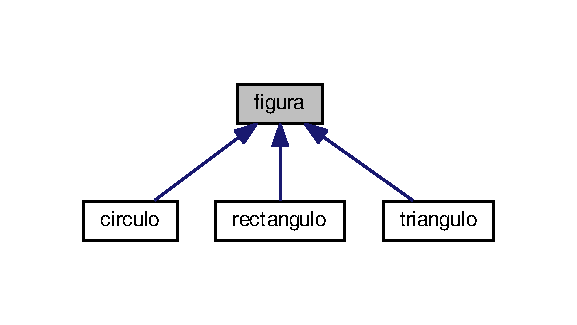
\includegraphics[width=277pt]{classfigura__inherit__graph}
\end{center}
\end{figure}
\subsection*{Public Member Functions}
\begin{DoxyCompactItemize}
\item 
\mbox{\Hypertarget{classfigura_a1496fac67d12bfc3ca8a1ed9cebdd49b}\label{classfigura_a1496fac67d12bfc3ca8a1ed9cebdd49b}} 
virtual void \hyperlink{classfigura_a1496fac67d12bfc3ca8a1ed9cebdd49b}{c\+\_\+area} ()=0
\begin{DoxyCompactList}\small\item\em función virtual c\+\_\+area utilizada para llamar a la función de area debida a la hora de correr el programa. \end{DoxyCompactList}\item 
\mbox{\Hypertarget{classfigura_a4e84ec7744c66ef59e35631485c34c4f}\label{classfigura_a4e84ec7744c66ef59e35631485c34c4f}} 
virtual void \hyperlink{classfigura_a4e84ec7744c66ef59e35631485c34c4f}{perimetro} ()=0
\begin{DoxyCompactList}\small\item\em funciónes virtuales c\+\_\+area utilizada para llamar a la función de perímetro debida a la hora de correr el programa. \end{DoxyCompactList}\item 
\mbox{\Hypertarget{classfigura_a8a33e4001eb52783bc6c04cdf32eedf6}\label{classfigura_a8a33e4001eb52783bc6c04cdf32eedf6}} 
virtual void \hyperlink{classfigura_a8a33e4001eb52783bc6c04cdf32eedf6}{info} ()=0
\begin{DoxyCompactList}\small\item\em funciónes virtuales c\+\_\+area utilizada para llamar a la identificacíon la hora de correr el programa. \end{DoxyCompactList}\end{DoxyCompactItemize}
\subsection*{Public Attributes}
\begin{DoxyCompactItemize}
\item 
\mbox{\Hypertarget{classfigura_a050e88ae9de6b6c82bcad928524ed8f5}\label{classfigura_a050e88ae9de6b6c82bcad928524ed8f5}} 
std\+::string {\bfseries name}
\item 
\mbox{\Hypertarget{classfigura_a2b187914ec19e6353658a6f8a6153623}\label{classfigura_a2b187914ec19e6353658a6f8a6153623}} 
std\+::string {\bfseries color}
\item 
\mbox{\Hypertarget{classfigura_a9cad6950721567dbd8655f941b373f38}\label{classfigura_a9cad6950721567dbd8655f941b373f38}} 
int {\bfseries id}
\end{DoxyCompactItemize}


The documentation for this class was generated from the following file\+:\begin{DoxyCompactItemize}
\item 
/home/moises/\+Documents/\+Estructuras de Datos/\+Labs/\+G3/\+Lab2/include/figura.\+h\end{DoxyCompactItemize}

\hypertarget{classrectangulo}{}\section{rectangulo Class Reference}
\label{classrectangulo}\index{rectangulo@{rectangulo}}


Inheritance diagram for rectangulo\+:\nopagebreak
\begin{figure}[H]
\begin{center}
\leavevmode
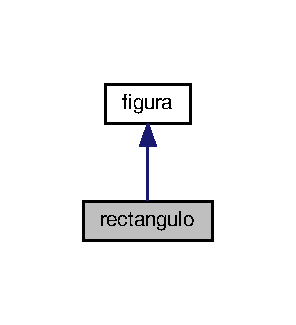
\includegraphics[width=142pt]{classrectangulo__inherit__graph}
\end{center}
\end{figure}


Collaboration diagram for rectangulo\+:\nopagebreak
\begin{figure}[H]
\begin{center}
\leavevmode
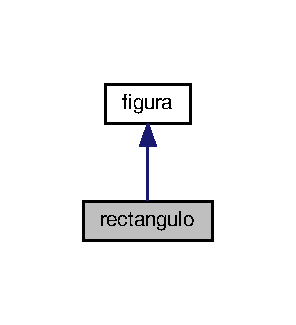
\includegraphics[width=142pt]{classrectangulo__coll__graph}
\end{center}
\end{figure}
\subsection*{Public Member Functions}
\begin{DoxyCompactItemize}
\item 
\hyperlink{classrectangulo_a0c066e0bfe8a56afe61d0b913864801c}{rectangulo} (double lado1, double lado2, int id, std\+::string nombre, std\+::string color)
\begin{DoxyCompactList}\small\item\em Función utilizada para llamar al constructor de la clase rectangulo. \end{DoxyCompactList}\item 
\mbox{\Hypertarget{classrectangulo_aba192e636fe037aaf0ccc294e4570b29}\label{classrectangulo_aba192e636fe037aaf0ccc294e4570b29}} 
\hyperlink{classrectangulo_aba192e636fe037aaf0ccc294e4570b29}{$\sim$rectangulo} ()
\begin{DoxyCompactList}\small\item\em Función la cual llama al destructor de rectangulo. \end{DoxyCompactList}\item 
\mbox{\Hypertarget{classrectangulo_a63ca5b15d7722d64280d94a7edc3ce65}\label{classrectangulo_a63ca5b15d7722d64280d94a7edc3ce65}} 
void \hyperlink{classrectangulo_a63ca5b15d7722d64280d94a7edc3ce65}{c\+\_\+area} ()
\begin{DoxyCompactList}\small\item\em Función heredada, para llamar al método que calcula el área del rectangulo. \end{DoxyCompactList}\item 
\mbox{\Hypertarget{classrectangulo_a493f8a9ea115164d439b6fd1d52a042d}\label{classrectangulo_a493f8a9ea115164d439b6fd1d52a042d}} 
void \hyperlink{classrectangulo_a493f8a9ea115164d439b6fd1d52a042d}{perimetro} ()
\begin{DoxyCompactList}\small\item\em Función heredada, para calcular el perímetro del rectangulo, multiplicando lado por lado. \end{DoxyCompactList}\item 
\mbox{\Hypertarget{classrectangulo_a0e632825c3e80d738625119454f1b9ce}\label{classrectangulo_a0e632825c3e80d738625119454f1b9ce}} 
void \hyperlink{classrectangulo_a0e632825c3e80d738625119454f1b9ce}{info} ()
\begin{DoxyCompactList}\small\item\em Función heredada, para imprimir la info del rectangulo a través de los parámetros miembros de la clase. \end{DoxyCompactList}\item 
sf\+::\+Convex\+Shape \hyperlink{classrectangulo_a43e4169c6127c4c6b58c54081b0370be}{dibujar} (sf\+::\+Render\+Window $\ast$rW)
\begin{DoxyCompactList}\small\item\em Función utilizada, para llamar al metodo que dibuja el rectángulo. \end{DoxyCompactList}\item 
\mbox{\Hypertarget{classrectangulo_a4cfd02cf92054992c583cc2f5a601c4c}\label{classrectangulo_a4cfd02cf92054992c583cc2f5a601c4c}} 
void \hyperlink{classrectangulo_a4cfd02cf92054992c583cc2f5a601c4c}{operator$\sim$} ()
\begin{DoxyCompactList}\small\item\em Función operador, para sobreescribir el simbolo $\sim$. \end{DoxyCompactList}\item 
\mbox{\Hypertarget{classrectangulo_a319b48b3d2a2229752f39a43a1c87d2c}\label{classrectangulo_a319b48b3d2a2229752f39a43a1c87d2c}} 
void \hyperlink{classrectangulo_a319b48b3d2a2229752f39a43a1c87d2c}{operator!} ()
\begin{DoxyCompactList}\small\item\em Función operador, para sobreescribir el simbolo !. \end{DoxyCompactList}\item 
\hyperlink{classrectangulo}{rectangulo} $\ast$ \hyperlink{classrectangulo_a7d8c56fe87e03931cefaa937b4d579ea}{operator=} (const \hyperlink{classrectangulo}{rectangulo} $\ast$t)
\begin{DoxyCompactList}\small\item\em metodo operador para un pointer de tipo rectangulo (clase), para sobreescribir el simbolo =. \end{DoxyCompactList}\item 
\mbox{\Hypertarget{classrectangulo_aac9d82c3854e707ae12c07eb377bcf10}\label{classrectangulo_aac9d82c3854e707ae12c07eb377bcf10}} 
int \hyperlink{classrectangulo_aac9d82c3854e707ae12c07eb377bcf10}{get\+\_\+num\+\_\+rectangulos} ()
\begin{DoxyCompactList}\small\item\em metodo get\+\_\+num\+\_\+rectangulos para obtener el numero de instancias de la clase rectangulo. \end{DoxyCompactList}\end{DoxyCompactItemize}
\subsection*{Public Attributes}
\begin{DoxyCompactItemize}
\item 
\mbox{\Hypertarget{classrectangulo_a7ed5010084a638538356fb8b3dabb34c}\label{classrectangulo_a7ed5010084a638538356fb8b3dabb34c}} 
sf\+::\+Convex\+Shape {\bfseries rect}
\end{DoxyCompactItemize}
\subsection*{Static Public Attributes}
\begin{DoxyCompactItemize}
\item 
\mbox{\Hypertarget{classrectangulo_ad046bab3349e76f167d01838aefe61d4}\label{classrectangulo_ad046bab3349e76f167d01838aefe61d4}} 
static int {\bfseries num\+\_\+rectangulos}
\end{DoxyCompactItemize}


\subsection{Constructor \& Destructor Documentation}
\mbox{\Hypertarget{classrectangulo_a0c066e0bfe8a56afe61d0b913864801c}\label{classrectangulo_a0c066e0bfe8a56afe61d0b913864801c}} 
\index{rectangulo@{rectangulo}!rectangulo@{rectangulo}}
\index{rectangulo@{rectangulo}!rectangulo@{rectangulo}}
\subsubsection{\texorpdfstring{rectangulo()}{rectangulo()}}
{\footnotesize\ttfamily rectangulo\+::rectangulo (\begin{DoxyParamCaption}\item[{double}]{lado1,  }\item[{double}]{lado2,  }\item[{int}]{id,  }\item[{std\+::string}]{nombre,  }\item[{std\+::string}]{color }\end{DoxyParamCaption})}



Función utilizada para llamar al constructor de la clase rectangulo. 


\begin{DoxyParams}{Parameters}
{\em lado1} & Tamaño del largo del rectangulo. \\
\hline
{\em lado2} & Tamaño del ancho del rectangulo. \\
\hline
{\em id} & numero que identifica a la instancia. \\
\hline
{\em nombre} & nombre de la instancia. \\
\hline
{\em color} & color del rectángulo, se muestra en la consola cuando corre el ejecutable. \\
\hline
\end{DoxyParams}


\subsection{Member Function Documentation}
\mbox{\Hypertarget{classrectangulo_a43e4169c6127c4c6b58c54081b0370be}\label{classrectangulo_a43e4169c6127c4c6b58c54081b0370be}} 
\index{rectangulo@{rectangulo}!dibujar@{dibujar}}
\index{dibujar@{dibujar}!rectangulo@{rectangulo}}
\subsubsection{\texorpdfstring{dibujar()}{dibujar()}}
{\footnotesize\ttfamily sf\+::\+Convex\+Shape rectangulo\+::dibujar (\begin{DoxyParamCaption}\item[{sf\+::\+Render\+Window $\ast$}]{rW }\end{DoxyParamCaption})}



Función utilizada, para llamar al metodo que dibuja el rectángulo. 


\begin{DoxyParams}{Parameters}
{\em $\ast$rW} & \+: puntero tipo Render\+Window en referencia a la clase del mismo nombre. \\
\hline
\end{DoxyParams}
\mbox{\Hypertarget{classrectangulo_a7d8c56fe87e03931cefaa937b4d579ea}\label{classrectangulo_a7d8c56fe87e03931cefaa937b4d579ea}} 
\index{rectangulo@{rectangulo}!operator=@{operator=}}
\index{operator=@{operator=}!rectangulo@{rectangulo}}
\subsubsection{\texorpdfstring{operator=()}{operator=()}}
{\footnotesize\ttfamily \hyperlink{classrectangulo}{rectangulo}$\ast$ rectangulo\+::operator= (\begin{DoxyParamCaption}\item[{const \hyperlink{classrectangulo}{rectangulo} $\ast$}]{t }\end{DoxyParamCaption})\hspace{0.3cm}{\ttfamily [inline]}}



metodo operador para un pointer de tipo rectangulo (clase), para sobreescribir el simbolo =. 


\begin{DoxyParams}{Parameters}
{\em rectangulo} & $\ast$t\+: un pointer que no modifica sus valores, para la lectura. \\
\hline
\end{DoxyParams}


The documentation for this class was generated from the following file\+:\begin{DoxyCompactItemize}
\item 
/home/moises/\+Documents/\+Estructuras de Datos/\+Labs/\+G3/\+Lab2/include/rectangulo.\+h\end{DoxyCompactItemize}

\hypertarget{classtriangulo}{}\section{triangulo Class Reference}
\label{classtriangulo}\index{triangulo@{triangulo}}


Inheritance diagram for triangulo\+:\nopagebreak
\begin{figure}[H]
\begin{center}
\leavevmode
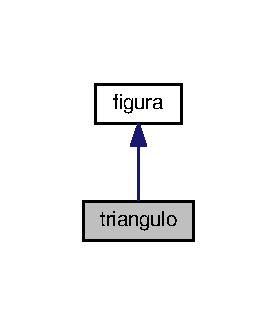
\includegraphics[width=133pt]{classtriangulo__inherit__graph}
\end{center}
\end{figure}


Collaboration diagram for triangulo\+:\nopagebreak
\begin{figure}[H]
\begin{center}
\leavevmode
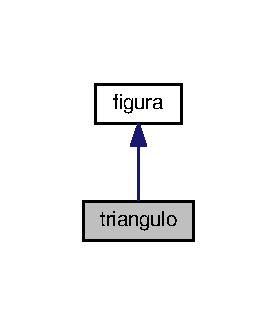
\includegraphics[width=133pt]{classtriangulo__coll__graph}
\end{center}
\end{figure}
\subsection*{Public Member Functions}
\begin{DoxyCompactItemize}
\item 
\hyperlink{classtriangulo_a0667fc13b900977472b1510da54848c5}{triangulo} (double lado, int id, std\+::string nombre, std\+::string color)
\begin{DoxyCompactList}\small\item\em Función utilizada para llamar al constructor de la clase triangulo. \end{DoxyCompactList}\item 
\mbox{\Hypertarget{classtriangulo_a8af9d6bbfd02ed3a82bd30147958ac34}\label{classtriangulo_a8af9d6bbfd02ed3a82bd30147958ac34}} 
\hyperlink{classtriangulo_a8af9d6bbfd02ed3a82bd30147958ac34}{$\sim$triangulo} ()
\begin{DoxyCompactList}\small\item\em Función utilizada para llamar al destructor de triangulo. \end{DoxyCompactList}\item 
\mbox{\Hypertarget{classtriangulo_a811c2e134e17a643bb7dce811c361b01}\label{classtriangulo_a811c2e134e17a643bb7dce811c361b01}} 
void \hyperlink{classtriangulo_a811c2e134e17a643bb7dce811c361b01}{c\+\_\+area} ()
\begin{DoxyCompactList}\small\item\em Función heredada, para llamar al método que calcula el área del triangulo. Toma en cuenta la mitad del lado y la altura mediante el método de Pitágoras. \end{DoxyCompactList}\item 
\mbox{\Hypertarget{classtriangulo_ad6ab43c962e747474bc155ca795fc1d8}\label{classtriangulo_ad6ab43c962e747474bc155ca795fc1d8}} 
void \hyperlink{classtriangulo_ad6ab43c962e747474bc155ca795fc1d8}{perimetro} ()
\begin{DoxyCompactList}\small\item\em Función heredada, para calcular el perímetro del triangulo. \end{DoxyCompactList}\item 
\mbox{\Hypertarget{classtriangulo_a0c489c6445ab778d8e6f4918bcc62649}\label{classtriangulo_a0c489c6445ab778d8e6f4918bcc62649}} 
void \hyperlink{classtriangulo_a0c489c6445ab778d8e6f4918bcc62649}{info} ()
\begin{DoxyCompactList}\small\item\em Función heredada, para imprimir la info del triangulo a través de los parámetros miembros de la clase. \end{DoxyCompactList}\item 
sf\+::\+Circle\+Shape \hyperlink{classtriangulo_a2fd521e84e1c22e67e7141ff66a81cd6}{dibujar} (sf\+::\+Render\+Window $\ast$rW)
\begin{DoxyCompactList}\small\item\em Función utilizada, para llamar al metodo que dibuja el triángulo. \end{DoxyCompactList}\item 
\mbox{\Hypertarget{classtriangulo_a62e3245477ae9ebd6023ac2cee4583b6}\label{classtriangulo_a62e3245477ae9ebd6023ac2cee4583b6}} 
void \hyperlink{classtriangulo_a62e3245477ae9ebd6023ac2cee4583b6}{operator$\sim$} ()
\begin{DoxyCompactList}\small\item\em Función operador, para sobreescribir el simbolo $\sim$. \end{DoxyCompactList}\item 
\mbox{\Hypertarget{classtriangulo_a9b0da9528de42b5f9bc12a96fbb93ddf}\label{classtriangulo_a9b0da9528de42b5f9bc12a96fbb93ddf}} 
void \hyperlink{classtriangulo_a9b0da9528de42b5f9bc12a96fbb93ddf}{operator!} ()
\begin{DoxyCompactList}\small\item\em Función operador, para sobreescribir el simbolo !. \end{DoxyCompactList}\item 
\hyperlink{classtriangulo}{triangulo} $\ast$ \hyperlink{classtriangulo_a0ed50f358a39886c852e30adb0bcaa7d}{operator=} (const \hyperlink{classtriangulo}{triangulo} $\ast$t)
\begin{DoxyCompactList}\small\item\em metodo operador para un pointer de tipo \hyperlink{classtriangulo}{triangulo( su clase)}, para sobreescribir el simbolo =. \end{DoxyCompactList}\item 
\mbox{\Hypertarget{classtriangulo_a0ac0e139c7cfe3cd3cd4f21d1284b446}\label{classtriangulo_a0ac0e139c7cfe3cd3cd4f21d1284b446}} 
int \hyperlink{classtriangulo_a0ac0e139c7cfe3cd3cd4f21d1284b446}{get\+\_\+num\+\_\+triangulos} ()
\begin{DoxyCompactList}\small\item\em metodo get\+\_\+num\+\_\+triangulos para obtener el numero de instancias de la clase triangulo. \end{DoxyCompactList}\end{DoxyCompactItemize}
\subsection*{Public Attributes}
\begin{DoxyCompactItemize}
\item 
sf\+::\+Circle\+Shape \hyperlink{classtriangulo_ad79b94dd36cc834a648db2f6b00a9c69}{tri}
\end{DoxyCompactItemize}
\subsection*{Static Public Attributes}
\begin{DoxyCompactItemize}
\item 
\mbox{\Hypertarget{classtriangulo_a6ae5ffe77b9a4ba1b9ed11ca3add3c83}\label{classtriangulo_a6ae5ffe77b9a4ba1b9ed11ca3add3c83}} 
static int {\bfseries num\+\_\+triangulos}
\end{DoxyCompactItemize}


\subsection{Constructor \& Destructor Documentation}
\mbox{\Hypertarget{classtriangulo_a0667fc13b900977472b1510da54848c5}\label{classtriangulo_a0667fc13b900977472b1510da54848c5}} 
\index{triangulo@{triangulo}!triangulo@{triangulo}}
\index{triangulo@{triangulo}!triangulo@{triangulo}}
\subsubsection{\texorpdfstring{triangulo()}{triangulo()}}
{\footnotesize\ttfamily triangulo\+::triangulo (\begin{DoxyParamCaption}\item[{double}]{lado,  }\item[{int}]{id,  }\item[{std\+::string}]{nombre,  }\item[{std\+::string}]{color }\end{DoxyParamCaption})}



Función utilizada para llamar al constructor de la clase triangulo. 


\begin{DoxyParams}{Parameters}
{\em lado} & Tamaño del lado del triangulo equilátero. \\
\hline
{\em id} & numero que identifica a la instancia. \\
\hline
{\em nombre} & nombre de la instancia. \\
\hline
{\em color} & color del triangulo, se muestra en la consola cuando corre el ejecutable. \\
\hline
\end{DoxyParams}


\subsection{Member Function Documentation}
\mbox{\Hypertarget{classtriangulo_a2fd521e84e1c22e67e7141ff66a81cd6}\label{classtriangulo_a2fd521e84e1c22e67e7141ff66a81cd6}} 
\index{triangulo@{triangulo}!dibujar@{dibujar}}
\index{dibujar@{dibujar}!triangulo@{triangulo}}
\subsubsection{\texorpdfstring{dibujar()}{dibujar()}}
{\footnotesize\ttfamily sf\+::\+Circle\+Shape triangulo\+::dibujar (\begin{DoxyParamCaption}\item[{sf\+::\+Render\+Window $\ast$}]{rW }\end{DoxyParamCaption})}



Función utilizada, para llamar al metodo que dibuja el triángulo. 


\begin{DoxyParams}{Parameters}
{\em $\ast$rW} & \+: puntero tipo Render\+Window en referencia a la clase del mismo nombre. \\
\hline
\end{DoxyParams}
\mbox{\Hypertarget{classtriangulo_a0ed50f358a39886c852e30adb0bcaa7d}\label{classtriangulo_a0ed50f358a39886c852e30adb0bcaa7d}} 
\index{triangulo@{triangulo}!operator=@{operator=}}
\index{operator=@{operator=}!triangulo@{triangulo}}
\subsubsection{\texorpdfstring{operator=()}{operator=()}}
{\footnotesize\ttfamily \hyperlink{classtriangulo}{triangulo}$\ast$ triangulo\+::operator= (\begin{DoxyParamCaption}\item[{const \hyperlink{classtriangulo}{triangulo} $\ast$}]{t }\end{DoxyParamCaption})\hspace{0.3cm}{\ttfamily [inline]}}



metodo operador para un pointer de tipo \hyperlink{classtriangulo}{triangulo( su clase)}, para sobreescribir el simbolo =. 


\begin{DoxyParams}{Parameters}
{\em triangulo} & $\ast$t\+: un pointer que no modifica sus valores, para la lectura. \\
\hline
\end{DoxyParams}


\subsection{Member Data Documentation}
\mbox{\Hypertarget{classtriangulo_ad79b94dd36cc834a648db2f6b00a9c69}\label{classtriangulo_ad79b94dd36cc834a648db2f6b00a9c69}} 
\index{triangulo@{triangulo}!tri@{tri}}
\index{tri@{tri}!triangulo@{triangulo}}
\subsubsection{\texorpdfstring{tri}{tri}}
{\footnotesize\ttfamily sf\+::\+Circle\+Shape triangulo\+::tri}

utlizamos la claase circle shape para hacer un polígono simple con su distancia al centro igual al \char`\"{}radio\char`\"{} para Circle\+Shape. 

The documentation for this class was generated from the following file\+:\begin{DoxyCompactItemize}
\item 
/home/moises/\+Documents/\+Estructuras de Datos/\+Labs/\+G3/\+Lab2/include/triangulo.\+h\end{DoxyCompactItemize}

%--- End generated contents ---

% Index
\backmatter
\newpage
\phantomsection
\clearemptydoublepage
\addcontentsline{toc}{chapter}{Index}
\printindex

\end{document}
